%\documentclass[spanish]{beamer}

\documentclass{beamer}
\usepackage{pgf,pgfpages}
%\pgfpagesuselayout{4 on 1}[letterpaper,landscape,border shrink=0.5in]
\usepackage{algorithm,algorithmic}
%\usepackage{algorithm,algorithmicx}
%\usepackage[noend]{algpseudocode}
\usepackage{listings}
\lstset{basicstyle=\ttfamily,
	showstringspaces=false,
	commentstyle=\color{red},
	literate={á}{{\'a}}1
	{ã}{{\~a}}1
	{é}{{\'e}}1
	{É}{{\'E}}1
	{ó}{{\'o}}1
	{í}{{\'i}}1
	{ñ}{{\~n}}1
	{¡}{{!`}}1
	{¿}{{?`}}1
	{ú}{{\'u}}1
	{Í}{{\'I}}1
	{Ó}{{\'O}}1
}

\usepackage{beamerthemesplit}
\usepackage{color}
\usepackage[utf8]{inputenc}
\usepackage[spanish]{babel}
%\usepackage[latin1]{inputenc}
%\usepackage[pdftex]{graphicx}
%\usepackage{algorithm}
%\usepackage{algorithmic-C}
%\usepackage{algorithmic}
\usepackage{amsthm}
\usepackage{multicol}
\usepackage{multirow}
\usepackage{fancyvrb,relsize}
\usepackage{hhline}
\usepackage{tikz}
\usetikzlibrary{trees, shapes, calc}
\newcommand{\inputTikZ}[2]{%
	\scalebox{#1}{\input{#2}}
}

\usetheme{Warsaw} %Gueno
%\usetheme{Darmstadt} %OK!
% \usetheme{Frankfurt} %OK!
%\usetheme{Goettingen}
%\usetheme{Dresden}
%\usetheme{JuanLesPins} %OK!!
%\usetheme{Marburg}
%\usetheme{Montpellier}
%\usetheme{Rochester} %sobrio
%\usetheme{Singapore}
%\usetheme{Szeged}

%\usecolortheme{albatross}
%\usecolortheme{seahorse}
%\usecolortheme{beetle}
%\usecolortheme{crane}
%\usecolortheme{dolphin}
%\usecolortheme{dove}
%\usecolortheme{fly}
%\usecolortheme{lily} %Gueno
\usecolortheme{orchid}%Gueno
%\usecolortheme{rose}
%\usecolortheme{seagull}
%\usecolortheme{whale}


\DefineVerbatimEnvironment%
      {VerbatimNN}%
      {Verbatim}%
      {fontsize=\relsize{-1}}
\DefineVerbatimEnvironment%
      {VerbatimNNN}%
      {Verbatim}%
      {fontsize=\relsize{-2}}

\DefineVerbatimEnvironment%
      {VerbatimPseudo}%
      {Verbatim}%
      {numbers=left, fontsize=\relsize{-1}}
\DefineVerbatimEnvironment%
      {VerbatimPseudoReduced}%
      {Verbatim}%
      {numbers=left, fontsize=\relsize{-2}}
\DefineVerbatimEnvironment%
      {VerbatimPseudoReduced2}%
      {Verbatim}%
      {numbers=left, fontsize=\relsize{-3}}
\DefineVerbatimEnvironment%
      {VerbatimC}%
      {Verbatim}%
      {commandchars=@ªº, numbers=left, fontsize=\relsize{-1}}
\DefineVerbatimEnvironment%
      {VerbatimReducedC}%
      {Verbatim}%
      {commandchars=@ªº, numbers=left, fontsize=\relsize{-2}}
\DefineVerbatimEnvironment%
      {VerbatimReduced2C}%
      {Verbatim}%
      {commandchars=@ªº, numbers=left, fontsize=\relsize{-3}}



%\AtBeginSubsection[]
%{
% \begin{frame}
% \frametitle{Sinopsis}
% Aqui decides: cada seccion y subseccion:
% \tableofcontents[currentsection,currentsubsection]
 %O solamente la seccion (Solo uno de ellos)
%\tableofcontents[currentsection]
% \end{frame}
%}

% Si quieres que todo por default aparezca de poco en poco
% descomenta esta linea
%\beamerdefaultoverlayspecification{<+->}

\setbeamertemplate{footline}{\hfill\insertframenumber/\inserttotalframenumber}
\setbeamertemplate{navigation symbols}{}

\setbeamercovered{transparent}

\title{ELO320 - Estructuras de Datos y Algoritmos\\Introducción a C\\Listas Doblemente Enlazadas}
%\subtitle{Ingeniería Civil Telemática UTFSM}
\author{Dr. Nicolás Gálvez R.\\{\small nicolas.galvez@usm.cl}}
\institute{Ing. Civil Telemática - Departamento de Electrónica}
\titlegraphic{
\includegraphics[scale=.18]{images/logoutfsm}}
\date{2do Semestre 2022}

\begin{document}

\frame{\titlepage}

%\section*{Sinopsis}
%\frame{  \frametitle{Sinopsis}\tableofcontents[pausesections]}
%
%

\section{Recordando: Lista Simple Enlazada}

\begin{frame}[fragile]
 \frametitle{Lista Simple Enlazada: Inicializar}

Las listas, en su versión más básica, dependen de un puntero al inicio de la lista. Éste suele llamarse \textit{header}, \textit{cabecera} o  \textit{inicio}.
\begin{exampleblock}{C}
\begin{lstlisting}[language=C, basicstyle=\tiny, escapeinside={|}{|}]
#include<stdio.h>

typedef struct nodo{
	int dato; //dato, puede ser lo que uds. necesiten
	struct nodo *sgte; // puntero a un nodo enalce.
} nodo_t;

int main(int argc, char **argv){

	nodo_t * inicio = NULL; 
	// Inicializamos la lista, con su puntero de inicio apuntando a NULL
	// Equivalente a lista vacía []

	return 0;
}
\end{lstlisting}
\end{exampleblock}
\end{frame}

\begin{frame}[fragile]
 \frametitle{Lista Simple Enlazada: Inicializar}
\begin{center}
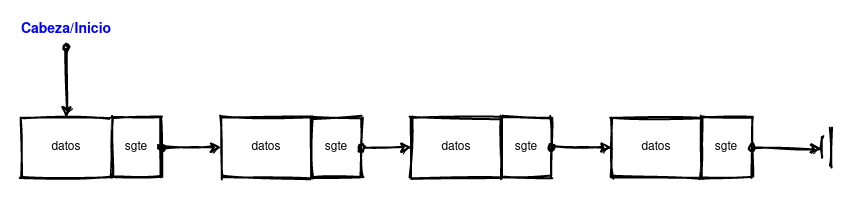
\includegraphics[width=.9\linewidth]{images/linkedlist1}
\end{center}

\begin{center}

\includegraphics[width=0.3\linewidth]{images/init1}
\end{center}
\end{frame}

\begin{frame}[fragile]
\frametitle{Lista Enlazada PRO}
Existen otras implementaciones de listas enlazadas simples, donde se incluyen más punteros y variables de control.

\begin{exampleblock}{C}
\begin{lstlisting}[language=C, basicstyle=\tiny, escapeinside={|}{|}]
#include<stdio.h>

typedef struct nodo{
	int dato; //dato, puede ser lo que uds. necesiten
	struct nodo *sgte; // puntero a un nodo enalce.
} nodo_t;

int main(int argc, char **argv){

	nodo_t * inicio = NULL; //pueden usar un struct para estos datos
	nodo_t * final = NULL;
	int largo = 0;
	// Equivalente a lista vacía []
	// ¿Para que sirve esta nueva forma?
	// Implemente las funciones de ésta clase considerando esta forma.

	return 0;
}
\end{lstlisting}
\end{exampleblock}
\end{frame}

\begin{frame}[fragile]
\frametitle{Lista Enlazada PRO}
\begin{center}
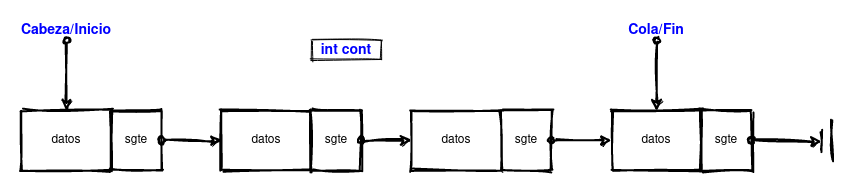
\includegraphics[width=.9\linewidth]{images/linkedlist2}
\end{center}


\begin{center}
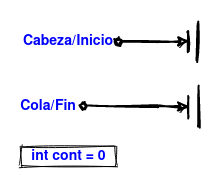
\includegraphics[width=.25\linewidth]{images/init2}
\end{center}

\end{frame}

\section{Lista Doblemente Enlazada}

\begin{frame}[fragile]
 \frametitle{Lista Doblemente Enlazada}

Una lista doblemente enlazada es una modificación de la lista simple enlazada. Éste TDA tiene un enlace más, para acceder rápidamente al nodo previo y tener una mejor nagevación sobre la estructura.
\begin{center}
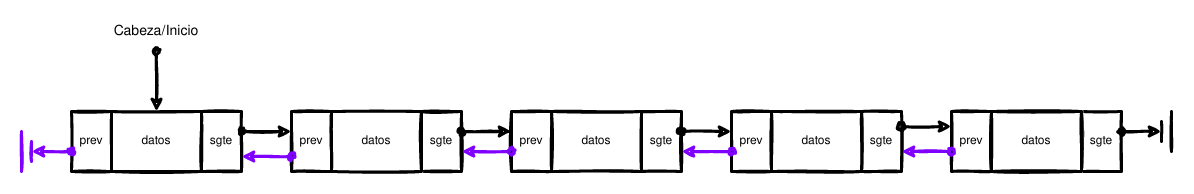
\includegraphics[width=\linewidth]{images/doublelinkedlist1}
\end{center}
Está compuesta por:
\begin{itemize}
\item Nodos: Contienen la información en lugares de memoria no ordenados.
\item Punteros: Enlazan los distintos nodos para conformar la lista.
\end{itemize}
\end{frame}

\begin{frame}[fragile]
 \frametitle{Lista Doblemente Enlazada}

Los punteros permiten al menos:
\begin{itemize}
\item Controlar el inicio de la lista.
\item Apuntar al siguiente elemento en la lista.
\item Apuntar al anterior elemento en la lista.
\item Acceder a cada nodo.  
\end{itemize}
\begin{center}
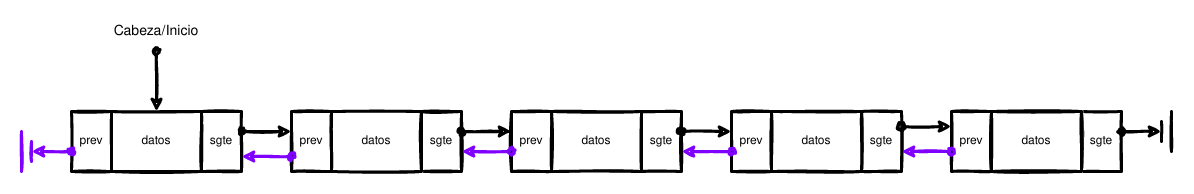
\includegraphics[width=\linewidth]{images/doublelinkedlist1}
\end{center}
\end{frame}

\begin{frame}[fragile]
 \frametitle{Lista Doblemente Enlazada: Nodos}

Los nodos son definidos con un struct, que almenos contiene un tipo de dato y un puntero. 

\begin{exampleblock}{C}
\begin{lstlisting}[language=C, basicstyle=\tiny, escapeinside={|}{|}]
struct nodo{
	int dato; //dato, puede ser lo que uds. necesiten
	struct nodo *sgte; // puntero a un nodo siguiente, enlace
	struct nodo *prev; // puntero a un nodo previo, enlace

};

typedef struct le_nodo{
	float datos[20]; //dato, puede ser lo que uds. necesiten
	struct le_nodo *sgte; // puntero a un nodo siguiente, enalce.
	struct le_nodo *prev; // puntero a un nodo previo, enalce.

} nodo_t;
\end{lstlisting}
\end{exampleblock}
\begin{center}
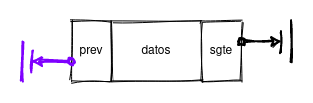
\includegraphics[width=.45\linewidth]{images/node_double}
\end{center}
\end{frame}


\begin{frame}[fragile]
 \frametitle{Lista Doblemente Enlazada: Interfaz}

Al igual que las listas simples enlazadas tienen un conjunto de funciones que interactúan como interfaz:
\begin{itemize}
\item Inicializar Lista. 
\item Agregar un elemento a una lista. 
\item Determinar el largo de una lista.
\item Eliminar un elemento de una lista.
\item Imprimir una lista. 
\item Limpiar una lista. 
\end{itemize}
\begin{center}
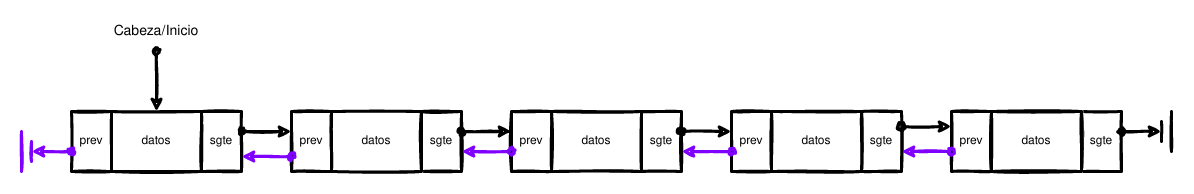
\includegraphics[width=\linewidth]{images/doublelinkedlist1}
\end{center}
\end{frame}

\begin{frame}[fragile]
 \frametitle{Lista Doblemente Enlazada: Inicializar}

Las listas, en su versión más básica, dependen de un puntero al inicio de la lista. Éste suele llamarse \textit{header}, \textit{cabecera} o  \textit{inicio}.
Las Listas Doblemente Enlazadas \textbf{siguen la misma dinámica} que las Listas Simple Enlazada.
\begin{exampleblock}{C}
\begin{lstlisting}[language=C, basicstyle=\tiny, escapeinside={|}{|}]
#include<stdio.h>

typedef struct nodo{
	int dato; //dato, puede ser lo que uds. necesiten
	struct nodo *sgte; // puntero a un nodo siguiente, enalce.
	struct nodo *prev; // puntero a un nodo previo, enalce.
} nodo_t;

int main(int argc, char **argv){

	nodo_t * inicio = NULL; 
	// Inicializamos la lista, con su puntero de inicio apuntando a NULL
	// Equivalente a lista vacía []

	return 0;
}
\end{lstlisting}
\end{exampleblock}

\begin{center}

\includegraphics[width=0.3\linewidth]{images/init1}
\end{center}
\end{frame}

\begin{frame}[fragile]
 \frametitle{Lista Doblemente Enlazada: Añadir nodos}

Esquema General:
\begin{center}
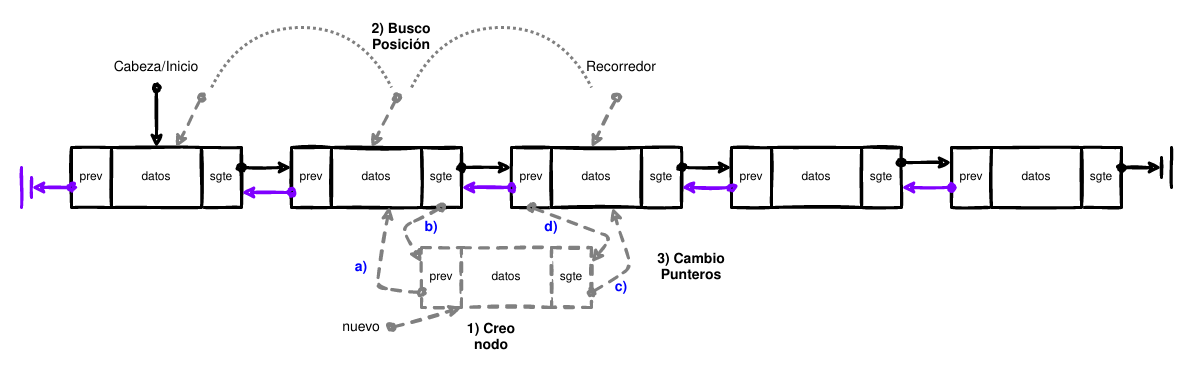
\includegraphics[width=\linewidth]{images/add_double1}
\end{center}

Debemos: 
\begin{enumerate}
\item<1> Crear el nodo \texttt{nuevo} y asignar el dato. 
\item<0> Buscar la posición a agregar el nodo. 
\item<0> Cambiar los punteros.
\end{enumerate}

\begin{itemize}
\item<0> Implemente esta función.
\item<0> ¿Qué precaución hay que tener si se quiere agregar al inicio o al final de la lista?
\end{itemize}

\end{frame}

\begin{frame}[fragile]
 \frametitle{Lista Doblemente Enlazada: Añadir nodos}

Esquema General:
\begin{center}
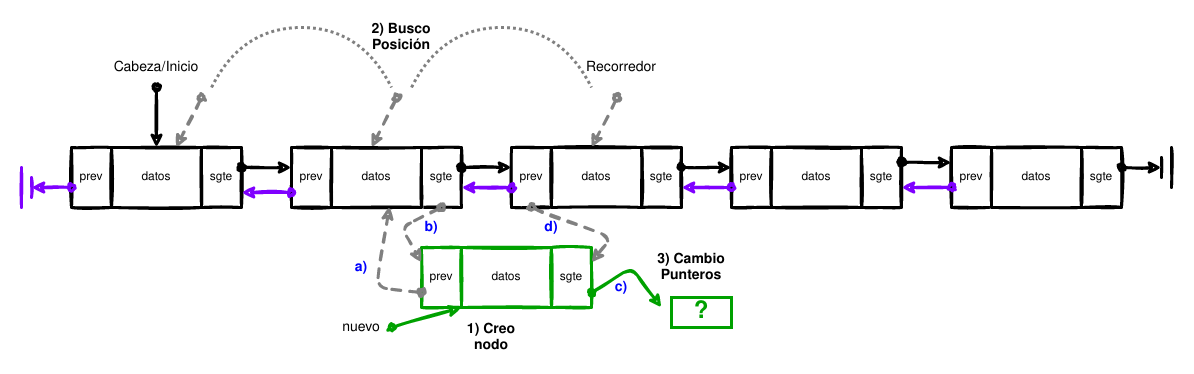
\includegraphics[width=\linewidth]{images/add_double2}
\end{center}

Debemos: 
\begin{enumerate}
\item<1> Crear el nodo \texttt{nuevo} y asignar el dato. 
\item<0> Buscar la posición a agregar el nodo. 
\item<0> Cambiar los punteros.
\end{enumerate}

\begin{itemize}
\item<0> Implemente esta función.
\item<0> ¿Qué precaución hay que tener si se quiere agregar al inicio o al final de la lista?
\end{itemize}

\end{frame}

\begin{frame}[fragile]
 \frametitle{Lista Doblemente Enlazada: Añadir nodos}

Esquema General:
\begin{center}
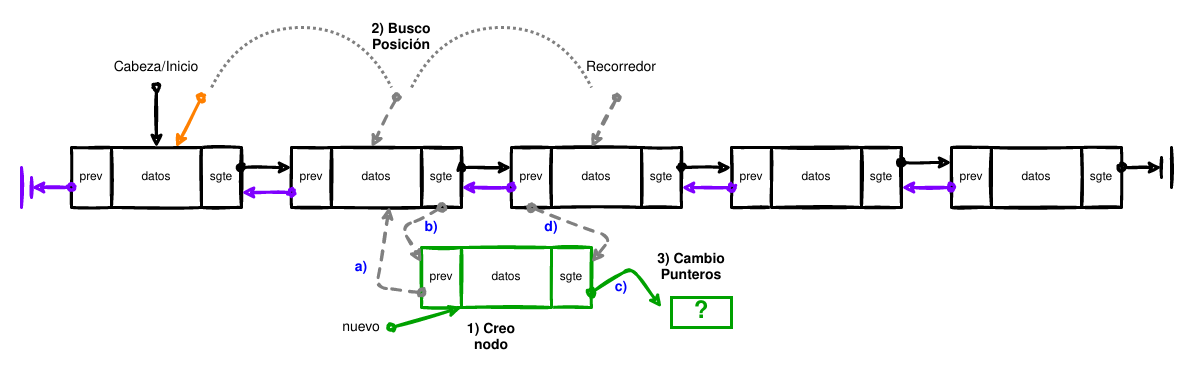
\includegraphics[width=\linewidth]{images/add_double3}
\end{center}

Debemos: 
\begin{enumerate}
\item<1> Crear el nodo \texttt{nuevo} y asignar el dato. 
\item<1> Buscar la posición a agregar el nodo. 
\item<0> Cambiar los punteros.
\end{enumerate}

\begin{itemize}
\item<0> Implemente esta función.
\item<0> ¿Qué precaución hay que tener si se quiere agregar al inicio o al final de la lista?
\end{itemize}

\end{frame}

\begin{frame}[fragile]
 \frametitle{Lista Doblemente Enlazada: Añadir nodos}

Esquema General:
\begin{center}
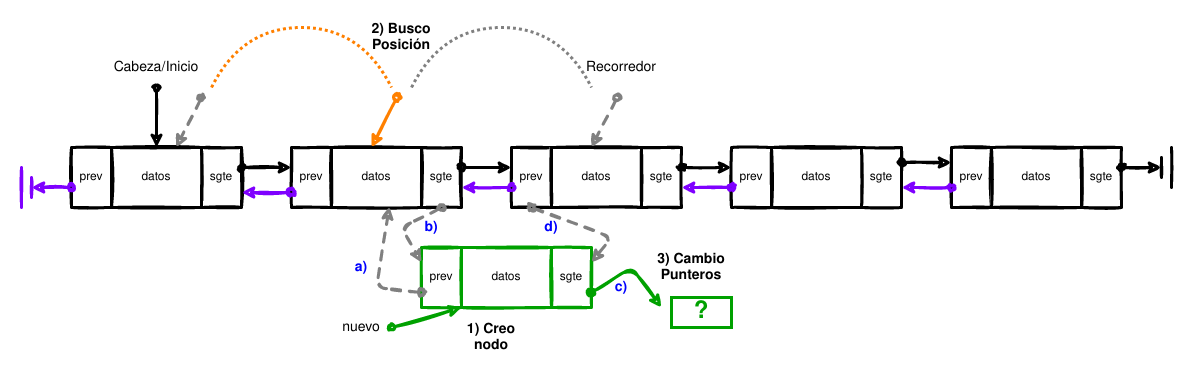
\includegraphics[width=\linewidth]{images/add_double4}
\end{center}

Debemos: 
\begin{enumerate}
\item<1> Crear el nodo \texttt{nuevo} y asignar el dato. 
\item<1> Buscar la posición a agregar el nodo. 
\item<0> Cambiar los punteros.
\end{enumerate}

\begin{itemize}
\item<0> Implemente esta función.
\item<0> ¿Qué precaución hay que tener si se quiere agregar al inicio o al final de la lista?
\end{itemize}

\end{frame}

\begin{frame}[fragile]
 \frametitle{Lista Doblemente Enlazada: Añadir nodos}

Esquema General:
\begin{center}
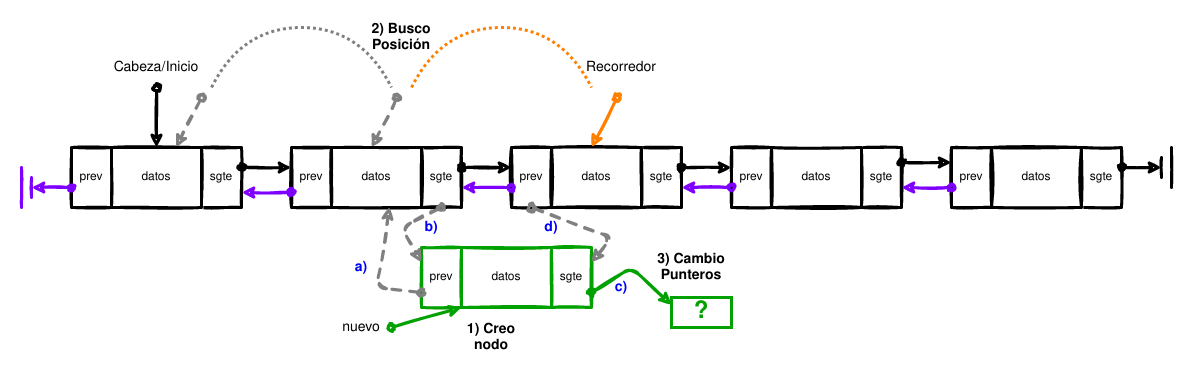
\includegraphics[width=\linewidth]{images/add_double5}
\end{center}

Debemos: 
\begin{enumerate}
\item<1> Crear el nodo \texttt{nuevo} y asignar el dato. 
\item<1> Buscar la posición a agregar el nodo. 
\item<0> Cambiar los punteros.
\end{enumerate}

\begin{itemize}
\item<0> Implemente esta función.
\item<0> ¿Qué precaución hay que tener si se quiere agregar al inicio o al final de la lista?
\end{itemize}

\end{frame}

\begin{frame}[fragile]
 \frametitle{Lista Doblemente Enlazada: Añadir nodos}

Esquema General:
\begin{center}
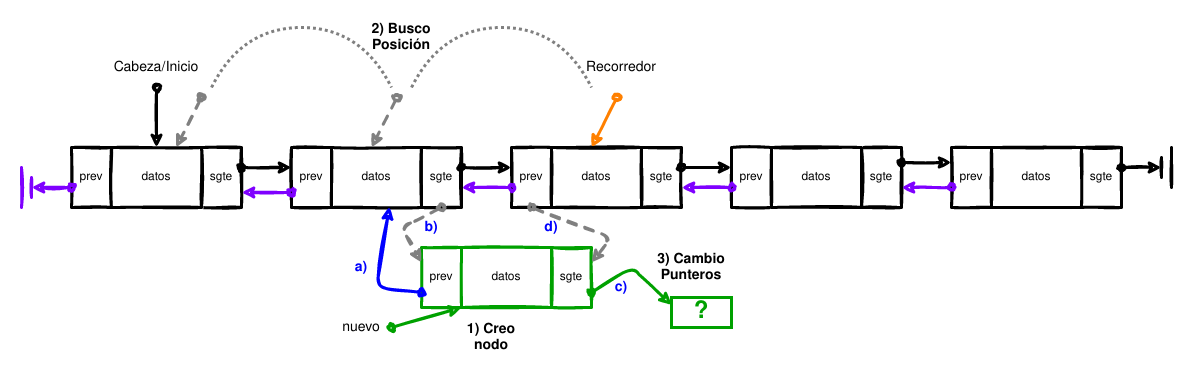
\includegraphics[width=\linewidth]{images/add_double6}
\end{center}

Debemos: 
\begin{enumerate}
\item<1> Crear el nodo \texttt{nuevo} y asignar el dato. 
\item<1> Buscar la posición a agregar el nodo. 
\item<1> Cambiar los punteros.
\end{enumerate}

\begin{itemize}
\item<0> Implemente esta función.
\item<0> ¿Qué precaución hay que tener si se quiere agregar al inicio o al final de la lista?
\end{itemize}

\end{frame}

\begin{frame}[fragile]
 \frametitle{Lista Doblemente Enlazada: Añadir nodos}

Esquema General:
\begin{center}
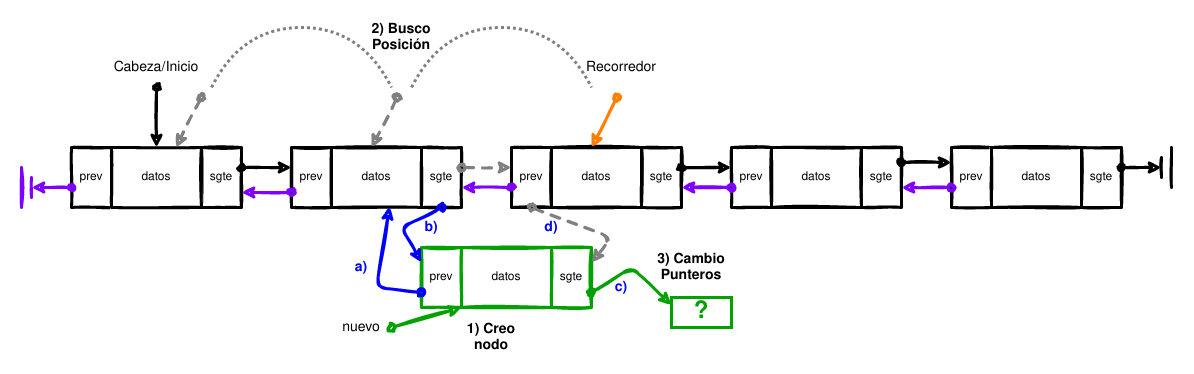
\includegraphics[width=\linewidth]{images/add_double7}
\end{center}

Debemos: 
\begin{enumerate}
\item<1> Crear el nodo \texttt{nuevo} y asignar el dato. 
\item<1> Buscar la posición a agregar el nodo. 
\item<1> Cambiar los punteros.
\end{enumerate}

\begin{itemize}
\item<0> Implemente esta función.
\item<0> ¿Qué precaución hay que tener si se quiere agregar al inicio o al final de la lista?
\end{itemize}

\end{frame}

\begin{frame}[fragile]
 \frametitle{Lista Doblemente Enlazada: Añadir nodos}

Esquema General:
\begin{center}
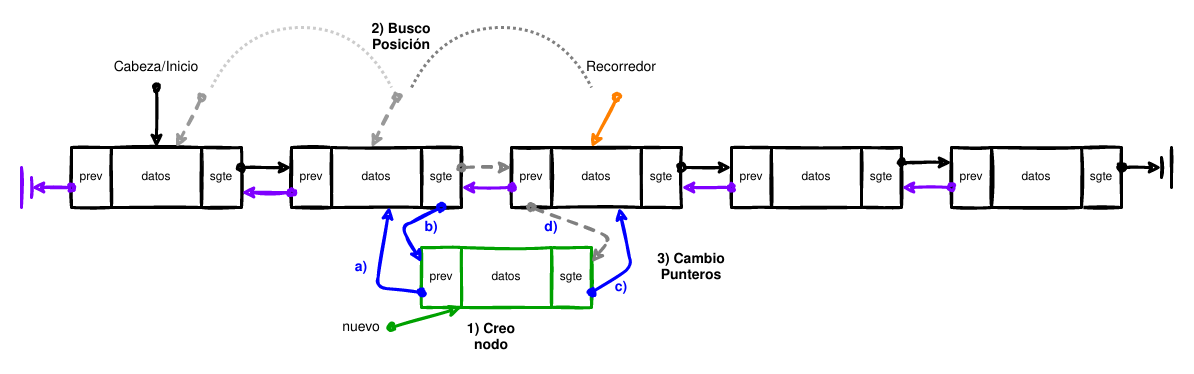
\includegraphics[width=\linewidth]{images/add_double8}
\end{center}

Debemos: 
\begin{enumerate}
\item<1> Crear el nodo \texttt{nuevo} y asignar el dato. 
\item<1> Buscar la posición a agregar el nodo. 
\item<1> Cambiar los punteros.
\end{enumerate}

\begin{itemize}
\item<0> Implemente esta función.
\item<0> ¿Qué precaución hay que tener si se quiere agregar al inicio o al final de la lista?
\end{itemize}

\end{frame}

\begin{frame}[fragile]
 \frametitle{Lista Doblemente Enlazada: Añadir nodos}

Esquema General:
\begin{center}
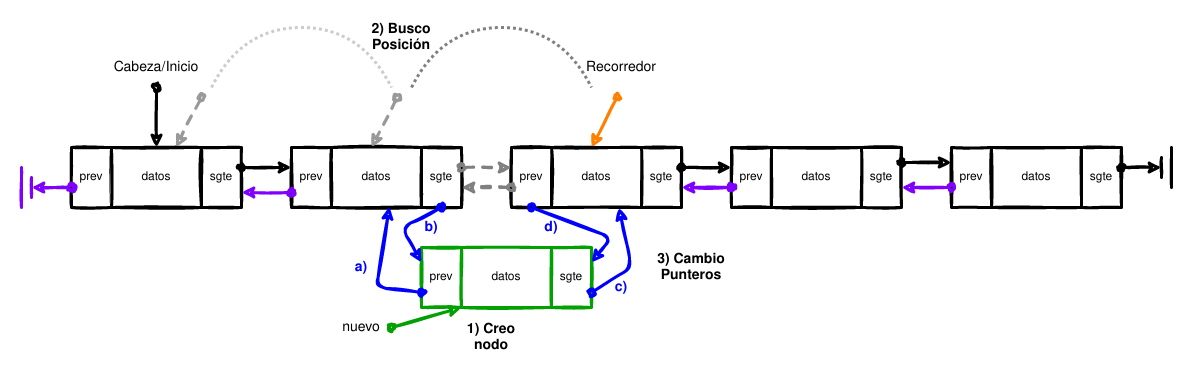
\includegraphics[width=\linewidth]{images/add_double9}
\end{center}

Debemos: 
\begin{enumerate}
\item<1> Crear el nodo \texttt{nuevo} y asignar el dato. 
\item<1> Buscar la posición a agregar el nodo. 
\item<1> Cambiar los punteros.
\end{enumerate}

\begin{itemize}
\item<1> Implemente esta función.
\item<1> ¿Qué precaución hay que tener si se quiere agregar al inicio o al final de la lista?
\end{itemize}

\end{frame}

\begin{frame}[fragile]
 \frametitle{Lista Doblemente Enlazada: Eliminar nodos}

Esquema General:
\begin{center}
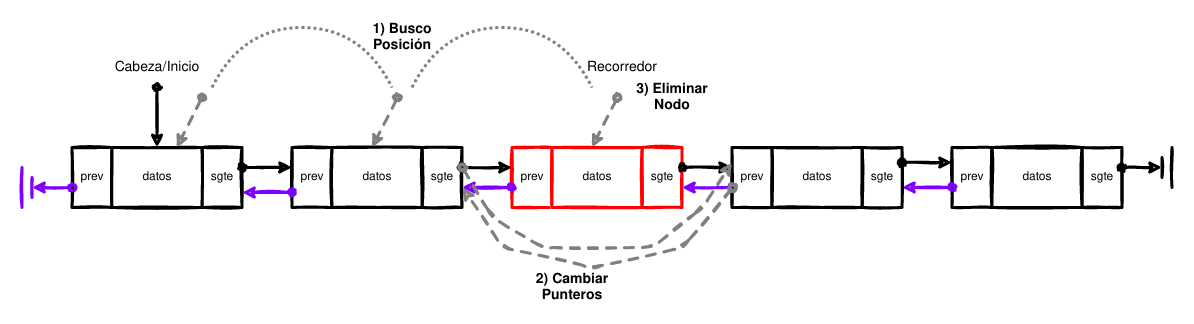
\includegraphics[width=\linewidth]{images/del_double1}
\end{center}

Ojo, que no siempre se pueden borrar nodos: \textbf{lista vacía}.

Debemos: 
\begin{enumerate}
\item<1> Buscar la posición del nodo a eliminar. 
\item<0> Cambiar los punteros.
\item<0> Eliminar el nodo. 
\end{enumerate}

\begin{itemize}
\item<0> Implemente esta función.
\item<0> ¿Qué precaución hay que tener si se quiere agregar al inicio o al final de la lista?
\end{itemize}
\end{frame}

\begin{frame}[fragile]
 \frametitle{Lista Doblemente Enlazada: Eliminar nodos}

Esquema General:
\begin{center}
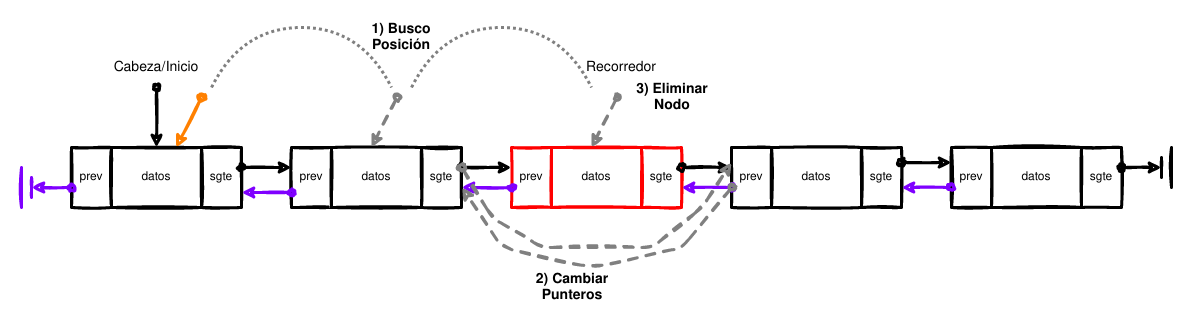
\includegraphics[width=\linewidth]{images/del_double2}
\end{center}

Ojo, que no siempre se pueden borrar nodos: \textbf{lista vacía}.

Debemos: 
\begin{enumerate}
\item<1> Buscar la posición del nodo a eliminar. 
\item<0> Cambiar los punteros.
\item<0> Eliminar el nodo. 
\end{enumerate}

\begin{itemize}
\item<0> Implemente esta función.
\item<0> ¿Qué precaución hay que tener si se quiere agregar al inicio o al final de la lista?
\end{itemize}
\end{frame}

\begin{frame}[fragile]
 \frametitle{Lista Doblemente Enlazada: Eliminar nodos}

Esquema General:
\begin{center}
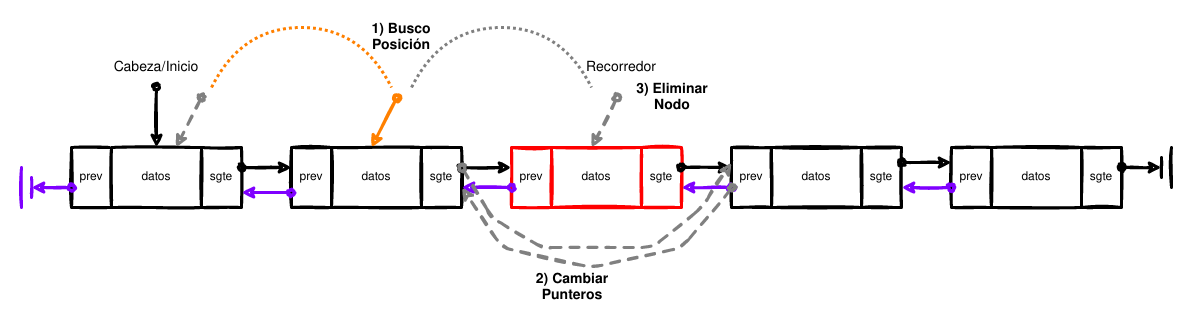
\includegraphics[width=\linewidth]{images/del_double3}
\end{center}

Ojo, que no siempre se pueden borrar nodos: \textbf{lista vacía}.

Debemos: 
\begin{enumerate}
\item<1> Buscar la posición del nodo a eliminar. 
\item<0> Cambiar los punteros.
\item<0> Eliminar el nodo. 
\end{enumerate}

\begin{itemize}
\item<0> Implemente esta función.
\item<0> ¿Qué precaución hay que tener si se quiere agregar al inicio o al final de la lista?
\end{itemize}
\end{frame}

\begin{frame}[fragile]
 \frametitle{Lista Doblemente Enlazada: Eliminar nodos}

Esquema General:
\begin{center}
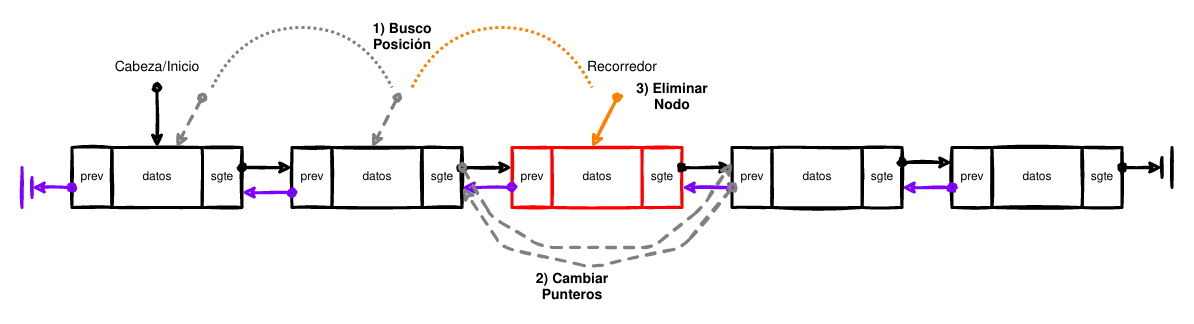
\includegraphics[width=\linewidth]{images/del_double4}
\end{center}

Ojo, que no siempre se pueden borrar nodos: \textbf{lista vacía}.

Debemos: 
\begin{enumerate}
\item<1> Buscar la posición del nodo a eliminar. 
\item<0> Cambiar los punteros.
\item<0> Eliminar el nodo. 
\end{enumerate}

\begin{itemize}
\item<0> Implemente esta función.
\item<0> ¿Qué precaución hay que tener si se quiere agregar al inicio o al final de la lista?
\end{itemize}
\end{frame}

\begin{frame}[fragile]
 \frametitle{Lista Doblemente Enlazada: Eliminar nodos}

Esquema General:
\begin{center}
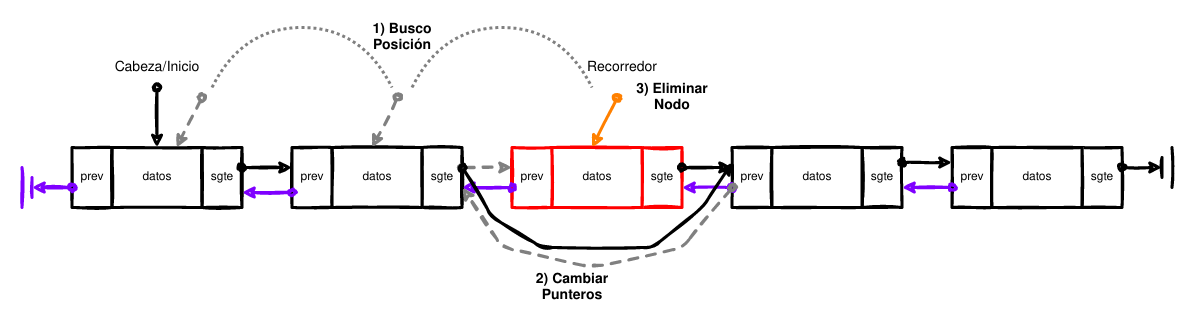
\includegraphics[width=\linewidth]{images/del_double5}
\end{center}

Ojo, que no siempre se pueden borrar nodos: \textbf{lista vacía}.

Debemos: 
\begin{enumerate}
\item<1> Buscar la posición del nodo a eliminar. 
\item<1> Cambiar los punteros.
\item<0> Eliminar el nodo. 
\end{enumerate}

\begin{itemize}
\item<0> Implemente esta función.
\item<0> ¿Qué precaución hay que tener si se quiere agregar al inicio o al final de la lista?
\end{itemize}
\end{frame}

\begin{frame}[fragile]
 \frametitle{Lista Doblemente Enlazada: Eliminar nodos}

Esquema General:
\begin{center}
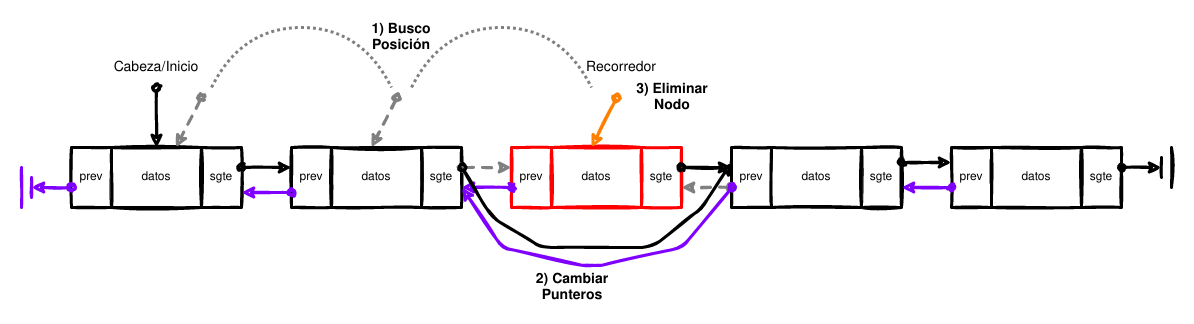
\includegraphics[width=\linewidth]{images/del_double6}
\end{center}

Ojo, que no siempre se pueden borrar nodos: \textbf{lista vacía}.

Debemos: 
\begin{enumerate}
\item<1> Buscar la posición del nodo a eliminar. 
\item<1> Cambiar los punteros.
\item<0> Eliminar el nodo. 
\end{enumerate}

\begin{itemize}
\item<0> Implemente esta función.
\item<0> ¿Qué precaución hay que tener si se quiere agregar al inicio o al final de la lista?
\end{itemize}
\end{frame}

\begin{frame}[fragile]
 \frametitle{Lista Doblemente Enlazada: Eliminar nodos}

Esquema General:
\begin{center}
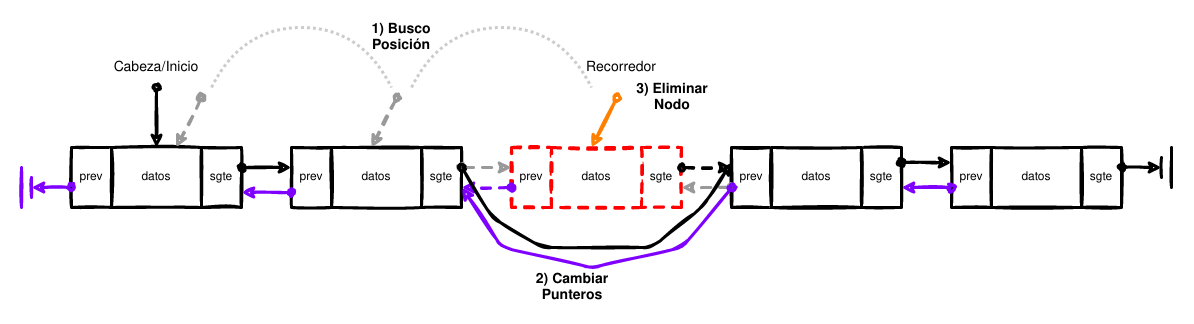
\includegraphics[width=\linewidth]{images/del_double7}
\end{center}

Ojo, que no siempre se pueden borrar nodos: \textbf{lista vacía}.

Debemos: 
\begin{enumerate}
\item<1> Buscar la posición del nodo a eliminar. 
\item<1> Cambiar los punteros.
\item<1> Eliminar el nodo. 
\end{enumerate}

\begin{itemize}
\item<1> Implemente esta función.
\item<1> ¿Qué precaución hay que tener si se quiere agregar al inicio o al final de la lista?
\end{itemize}
\end{frame}


\begin{frame}[fragile]
 \frametitle{Lista Doblemente Enlazada: Funciones.}
Basado en las conocidas funciones de Listas Simples Enlazadas, implemente las siguientes funciones para Listas Doblemente enlazadas:
\begin{itemize}
\item Determinar el largo de una lista.
\item Imprimir una lista. 
\item Limpiar una lista. 
\end{itemize}

\end{frame}


\section{Mejora: Lista Doblemente Enlazada PRO}
\begin{frame}[fragile]
\frametitle{Lista Doblemente Enlazada PRO}
Existen otras implementaciones de listas enlazadas simples, donde se incluyen más punteros y variables de control.

\begin{exampleblock}{C}
\begin{lstlisting}[language=C, basicstyle=\tiny, escapeinside={|}{|}]
#include<stdio.h>

typedef struct nodo{
	int dato; //dato, puede ser lo que uds. necesiten
	struct nodo *sgte; // puntero a un nodo enalce.
} nodo_t;

int main(int argc, char **argv){

	nodo_t * inicio = NULL; //pueden usar un struct para estos datos
	nodo_t * final = NULL;
	int largo = 0;
	// Equivalente a lista vacía []
	// ¿Para que sirve esta nueva forma?
	// Implemente las funciones de ésta clase considerando esta forma.

	return 0;
}
\end{lstlisting}
\end{exampleblock}
\end{frame}

\begin{frame}[fragile]
\frametitle{Lista Doblemente Enlazada PRO}
\begin{center}
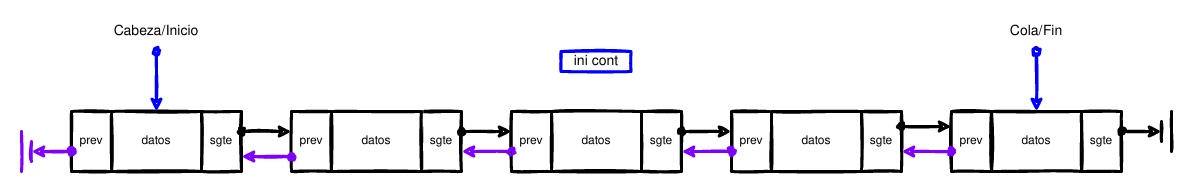
\includegraphics[width=\linewidth]{images/doublelinkedlist2}
\end{center}
\end{frame}

\begin{frame}[fragile]
\frametitle{Lista Doblemente Enlazada PRO+}
Existen otras implementaciones de listas enlazadas simples, donde se incluyen más punteros y variables de control.

\begin{exampleblock}{C}
\begin{lstlisting}[language=C, basicstyle=\tiny, escapeinside={|}{|}]
#include<stdio.h>

typedef struct nodo{
	int dato; //dato, puede ser lo que uds. necesiten
	struct nodo *sgte; // puntero a un nodo enalce.
} nodo_t;

int main(int argc, char **argv){

	nodo_t * inicio = NULL; //pueden usar un struct para estos datos
	nodo_t * final = NULL;
	nodo_t * actual = NULL;
	int largo = 0;
	int pos_actual = 0;
	// Equivalente a lista vacía []
	// ¿Para que sirve esta nueva forma?
	// Implemente las funciones de ésta clase considerando esta forma.

	return 0;
}
\end{lstlisting}
\end{exampleblock}
\end{frame}


\begin{frame}[fragile]
\frametitle{Lista Doblemente Enlazada PRO+}
\begin{center}
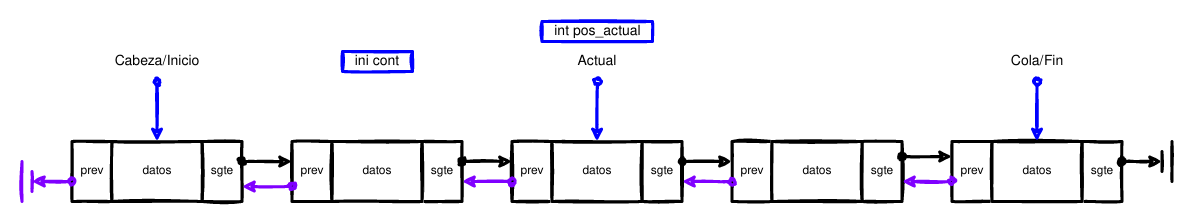
\includegraphics[width=\linewidth]{images/doublelinkedlist3}
\end{center}
\end{frame}

\section{Otras Listas}



\section{Ejercicio: Construyendo la lista de Python en C}
\begin{frame}[fragile]
\frametitle{Lista de Python en C}

Implemente una lista de cada tipo; Simple, Simple PRO, Doble, Doble PRO, Doble PRO+; para algún tipo de dato a su elección, que incluya las funciones más conocidas de las listas de Python:

\begin{itemize}
\item \texttt{list()} o \text{[]}.
\item \texttt{.insert(pos, value)}
\item \texttt{.append(value)}
\item \texttt{.clear()}
\item \texttt{del lista[pos]}
\item \texttt{.remove(value)}
\item \texttt{.sort()}
\item \texttt{.reverse()}
\item \texttt{.count(value)}
\item \texttt{.index(value)}
\end{itemize}

\end{frame}

\end{document}
